\documentclass[review]{elsarticle}
\usepackage{float}
\usepackage{lineno}
\usepackage{hyperref}
\urlstyle{same}
\usepackage[version=3]{mhchem}
\usepackage{textcomp}
\usepackage{gensymb}
\usepackage[utf8]{inputenc}
\usepackage{graphicx}
\usepackage{mathtools}
\modulolinenumbers[5]


\usepackage{nomencl}
\makenomenclature


% Replaces journal with pagenumber
\makeatletter
\def\ps@pprintTitle{%
 \let\@oddhead\@empty
 \let\@evenhead\@empty
 \def\@oddfoot{\centerline{\thepage}}%
 \let\@evenfoot\@oddfoot}
\makeatother
% \journal{ } 

%%%%%%%%%%%%%%%%%%%%%%%
%% Elsevier bibliography styles
%%%%%%%%%%%%%%%%%%%%%%%
%% To change the style, put a % in front of the second line of the current style and
%% remove the % from the second line of the style you would like to use.
%%%%%%%%%%%%%%%%%%%%%%%

%% Numbered
%\bibliographystyle{model1-num-names}

%% Numbered without titles
%\bibliographystyle{model1a-num-names}

%% Harvard
%\bibliographystyle{model2-names.bst}\biboptions{authoryear}

%% Vancouver numbered
%\usepackage{numcompress}\bibliographystyle{model3-num-names}

%% Vancouver name/year
%\usepackage{numcompress}\bibliographystyle{model4-names}\biboptions{authoryear}

%% APA style
%\bibliographystyle{model5-names}\biboptions{authoryear}

%% AMA style
%\usepackage{numcompress}\bibliographystyle{model6-num-names}

%% `Elsevier LaTeX' style
\bibliographystyle{elsarticle-num}
%%%%%%%%%%%%%%%%%%%%%%%

\begin{document}

\begin{frontmatter}

\title{}

%% Group authors per affiliation:
\author{Peter Armstrong}
\address{University College Cork - 115224113 \\ Cork Institute of Technology - R00145003 }

\begin{abstract}


The aim of this project was to model the heat transfer through a cooling rod using the finite volume method.
The 1D heat transfer equation was used to model the temperature distribution.
The equations for the cooling fin were manually developed for a three node grid. These equations were then solved in a python script to calculate temperature values at each node. Three different grid sizes were compared and the results for each grid are compared with the analytical solution. 
The temperatures found at the end of the cooling rod using the different methods were within 1\degree C of each other. The temperatures calculated for areas close to the base of the cooling rod varied widely depending on grid sizes. A coarse mesh is sufficient if the end temperature is the only parameter of interest. A finer mesh is needed to accurately model the temperature distribution along the length of the fin.


% TODO: Insert major results / conclusions.
% Aims
% Methods
% Key Results
% Major Conclusions

\end{abstract}

% \begin{keyword}
% \texttt{elsarticle.cls}\sep \LaTeX\sep Elsevier \sep template
% \MSC[2010] 00-01\sep  99-00
% \end{keyword}

% TOC

% Nomenclature

% Introduction
% Background information
% Aim - problem statement
% develop objectives - specific tasks to meet the aim


% Main body
% In detail development of methods
% Justify engineering solutions
% Crucial to credibility of work
% Results
% discussion

% Ending
% Conclusions - consise. Bullet points may be appropriate. Link back to aims in introduction
% Recommendations

% Discuss images / tables before they are presented

\end{frontmatter}

\linenumbers

\printnomenclature
\section{Introduction}

Cooling fins are used in many devices where heat needs to be dissipated from a heat source. Car radiators and computer processor heatsinks both incorporate cooling fins. They cool the heat source by increasing the surface area available for convective heat transfer. It is important to accurately model the heat transfer through a cooling fin.

In this analysis, a circular section cooling fin as in figure \ref{fin} is attached to a heat source at a temperature \(T_{B}\) of 250\degree C. The other end of the fin is insulated. Heat is lost to the ambient temperature \(T_\infty\) of 20\degree C. The length of the fin L is 1.5m.
The heat transfer coefficient h, perimeter of the fin P, cross sectional area of the fin A and thermal conductivity of the fin material k are such that:

\[ \frac{hP}{kA} = n^{2} = 25 \]

\begin{figure}[H]
    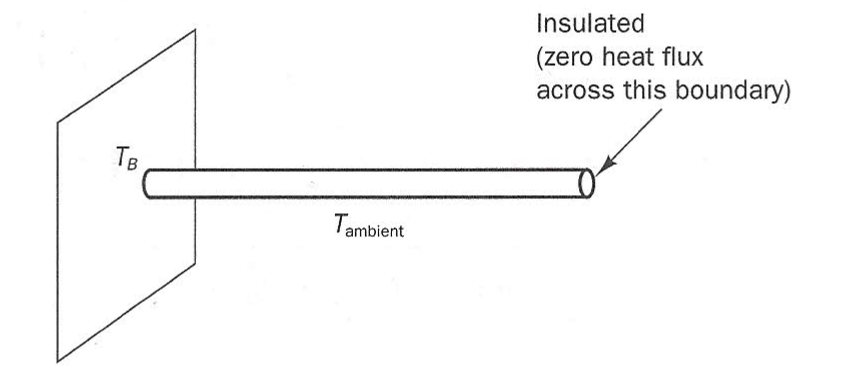
\includegraphics[width=\textwidth]{img/cooling_fin.png}
    \caption{Cooling Fin}
    \label{fin}
\end{figure}

\section{Finite Volume Method}
The finite volume method 1D heat transfer is governed by the equation:

\[ \frac{d}{dx} \left(kA \frac{dT}{dx} \right) - hp(T - T_{\infty}) = 0 \]

This can be rewritten as:
\[ \frac{d}{dx} \left(\frac{dT}{dx} \right) - n^2(T - T_{\infty}) = 0 \]

Integrate over the control volume:

\[\int\limits_{\Delta V} \frac{d}{dx}\left(\frac{dT}{dx} \right) dV - \int\limits_{\Delta V} n^2(T-T_{\infty}) dV  = 0\]


\[ \left[ \left(A \frac{dT}{dx} \right)_{eastface} - \left(A \frac{dT}{dx} \right)_{westface} \right] - (n^2 (T_P - T_{\infty})Adx) = 0 \]

\( \frac{dT}{dx} \) for the east face of a node can be written as \( \frac{T_E - T_P}{dx}\), and the west face as \( \frac{T_P - T_W}{dx} \), where \(T_{E}\) is the temperature of the node to the east, \(T_{W}\) the temperature of the node to the west and \(T_{P}\) the temperature of the node in question.

Divide across by A, and rearrange:
\[ - \left(\frac{1}{dx}\right)T_W + \left(\frac{2}{dx} + n^{2}dx\right)T_P - \left(\frac{1}{dx}\right)T_E = n^2dxT_{\infty} \]

The equation in this form is suitable for nodes with a node both to the west and to the east. For the first and last nodes, the equation will need to be modified, as either \(T_E\) or \(T_W\) is not available.

\subsection{First Node}
The first node does not have a node to the west. Instead, we know the temperature of the west face - the temperature of the base of the cooling fin, \(T_B\). The temperature change at the west face occurs over half a node, so the formula is modified:

\[ \left[ \left( \frac{T_E - T_P}{dx} \right) - \left( \frac{T_P - T_B}{dx/2} \right) \right] - (n^2 (T_P - T_{\infty})dx) = 0 \]

This can be rearranged to:

\[ \left(\frac{3}{dx} + n^{2}dx\right)T_P - \left(\frac{1}{dx}\right)T_E = n^2dxT_{\infty} + 2 \frac{T_B}{dx} \]



\subsection{Last Node}
The last node does not have a node to the east. We know that the end of the rod is insulated - there is no flux across the boundary - \(\left(\frac{dT}{dx} \right)_{eastface} = 0 \).

Our formula is modified:
\[ \left[ - \left( \frac{T_P - T_W}{dx} \right) \right] - (n^2 (T_P - T_{\infty})dx) = 0 \]


\[ - \left(\frac{1}{dx}\right)T_W + \left(\frac{1}{dx} + n^{2}dx\right)T_P  = n^2dxT_{\infty} \]



By applying these formulas to each node, a series of simultaneous equations can be generated. There will be the same number of equations as the number of unknown temperature values, so the equations can be solved.
A python script was used to solve for each value of T.

\section{Analytical Method}

An analytical solution for the problem can be calculated using the formula:

\[\frac{T- T_{\infty}}{T_{B} - T_{\infty}} = \frac{cosh(n(L-x))}{cosh(nL)} \]

In this case, the value for T at each node was calculated using a python script.


\section{Results}

\subsection{3 Node Grid}

\begin{center}
  \begin{tabular}{| l | c | c | c |}
    \hline
    Node & Analytical & FVM & \% error \\ \hline
    1 & 85.9 & 70.4 & 18.0 \\
    2 & 25.4 & 26.2 & -3.2 \\
    3 & 20.5 & 20.9 & -1.8 \\
    \hline
  \end{tabular}
\end{center}

\begin{figure}[H]
    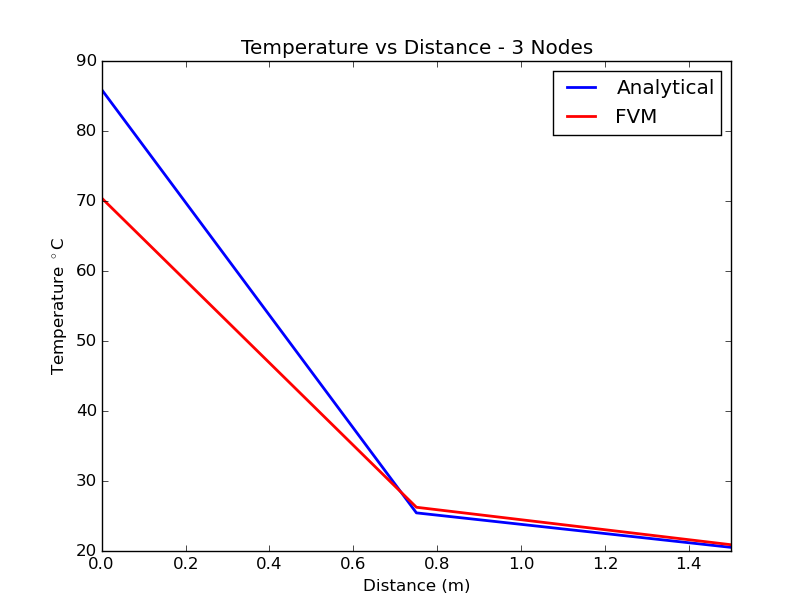
\includegraphics[width=\textwidth]{img/3_nodes_avsf.png}
    \caption{Analytical vs FVM - 3 Nodes}
    \label{3nodes}
\end{figure}

\subsection{6 Node Grid}
\begin{center}
  \begin{tabular}{| l | c | c | c |}
    \hline
    Node & Analytical & FVM & \% error \\ \hline
    1 & 143.1 & 128.1 & 10.5 \\
    2 & 55.3 & 53.2 & 3.7 \\
    3 & 30.1 & 30.2 & -0.3 \\
    4 & 22.9 & 23.1 & -1.1 \\ 
    5 & 20.8 & 21.0 & -0.7 \\
    6 & 20.3 & 20.4 & -0.4 \\
    \hline
  \end{tabular}
\end{center}

\begin{figure}[H]
    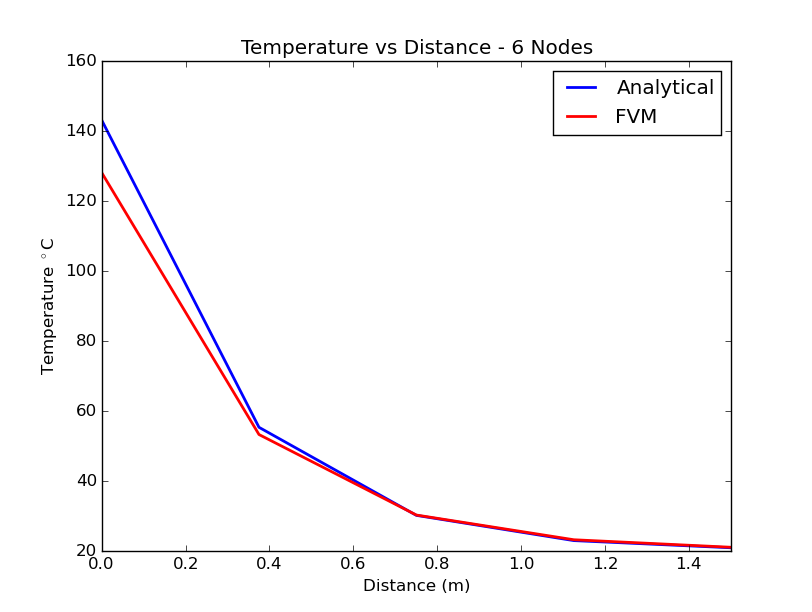
\includegraphics[width=\textwidth]{img/6_nodes_avsf.png}
    \caption{Analytical vs FVM - 6 Nodes}
    \label{6nodes}
\end{figure}

\subsection{15 Node Grid}

\begin{center}
  \begin{tabular}{| l | c | c | c |}
    \hline
    Node & Analytical & FVM & \% error \\ \hline
    1 & 199.1 & 194.2 & 2.5 \\
    2 & 128.6 & 126.2 & 1.9 \\
    3 & 85.9  & 84.7  & 1.3 \\
    4 & 60.0  & 59.5  & 0.8 \\
    5 & 44.2  & 44.1  & 0.4 \\
    6 & 34.7  & 34.7  & 0.1 \\
    7 & 28.9  & 28.9  & -0.1  \\
    8 & 25.4  & 25.5  & -0.2  \\
    9 & 23.3  & 23.3  & -0.2  \\
    10  & 22.0  & 22.0  & -0.2  \\
    11  & 21.2  & 21.2  & -0.1  \\
    12  & 20.8  & 20.8  & -0.1  \\
    13  & 20.5  & 20.5  & -0.1  \\
    14  & 20.3  & 20.3  & -0.1  \\
    15  & 20.3  & 20.3  & -0.1  \\
    \hline
  \end{tabular}
\end{center}

\begin{figure}[H]
    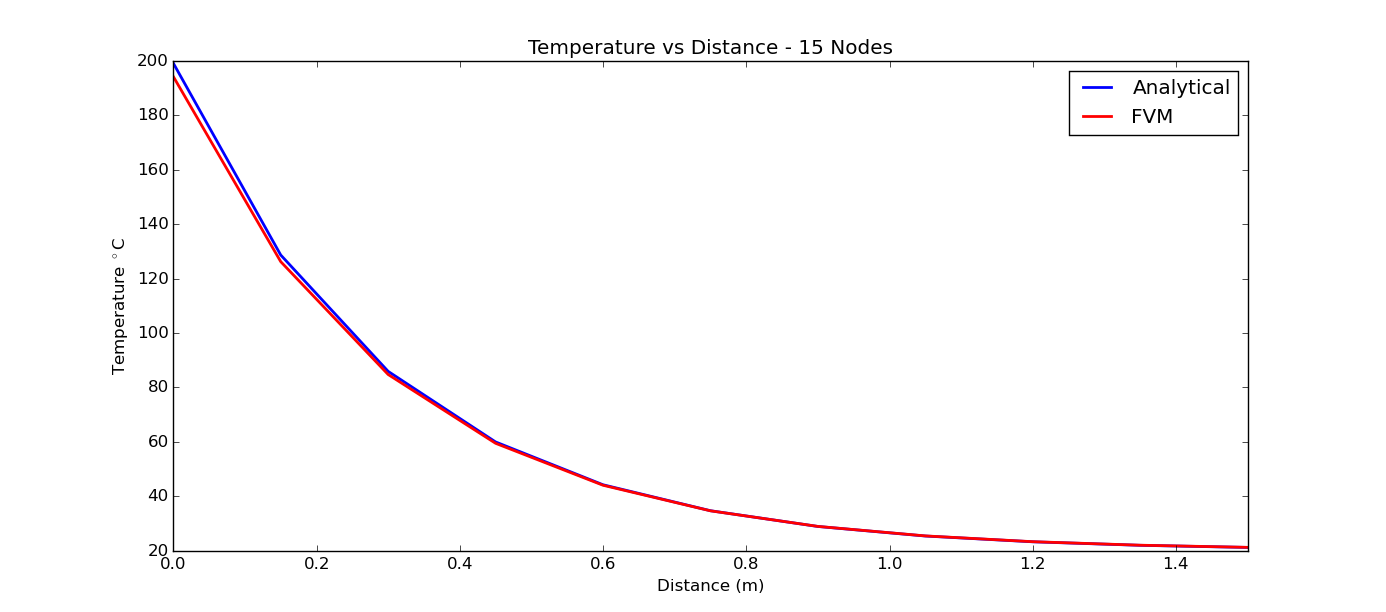
\includegraphics[width=\textwidth]{img/15_nodes_avsf.png}
    \caption{Analytical vs FVM - 15 Nodes}
    \label{15nodes}
\end{figure}



\section{Conclusion}

\begin{itemize}
  \item A grid with more nodes produces a more accurate solution.
  \item Each grid gives an temperature at the end of the cooling fin within 1\degree C.
  \item The error between the analytical solution and the finite volume solution is within 1\degree C at the end of the cooling fin.
  \item The error near the base of the fin is much greater. The 3-node grid gives an error of over 15\degree C (18\%) at the first node. The 15-node grid improves this error to just 5\degree C (2.5\%). This is to be expected as the temperature gradient is largest at the base of the cooling fin.
  \item Computational time is not noticeably increased when using a 15-node grid versus a 3-node grid.
\end{itemize}

\subsection{Recommendations}
\begin{itemize}
  \item If accuracy near the base of the cooling fin is important, a fine mesh is needed.
  \item If temperature at the end of the fin is the only parameter of interest, a coarse mesh is sufficient.
\end{itemize}


\nomenclature{\(T_B\)}{Temperature at base of fin}
\nomenclature{\(T_{\infty}\)}{Ambient temperature}
\nomenclature{\(T_P\)}{Temperature at node P, the node in question}
\nomenclature{\(T_E\)}{Temperature at the node to the east of node P}
\nomenclature{\(T_W\)}{Temperature at the node to the west of node P}
\nomenclature{T}{Temperature of fin at distance along the fin}
\nomenclature{x}{Distance along the fin}
\nomenclature{h}{Heat transfer coefficient}
\nomenclature{P}{Perimeter of cooling fin}
\nomenclature{A}{Cross sectional area of cooling fin}
\nomenclature{k}{Thermal conductivity of fin material}
\nomenclature{dx}{Width of grid element. Length / grid size}
\nomenclature{L}{Length of cooling fin}

% \section*{References}

% \bibliography{bib}

\end{document}